\documentclass[11pt]{article}

    \usepackage[breakable]{tcolorbox}
    \usepackage{parskip} % Stop auto-indenting (to mimic markdown behaviour)
    
    \usepackage{iftex}
    \ifPDFTeX
    	\usepackage[T1]{fontenc}
    	\usepackage{mathpazo}
    \else
    	\usepackage{fontspec}
    \fi

    % Basic figure setup, for now with no caption control since it's done
    % automatically by Pandoc (which extracts ![](path) syntax from Markdown).
    \usepackage{graphicx}
    % Maintain compatibility with old templates. Remove in nbconvert 6.0
    \let\Oldincludegraphics\includegraphics
    % Ensure that by default, figures have no caption (until we provide a
    % proper Figure object with a Caption API and a way to capture that
    % in the conversion process - todo).
    \usepackage{caption}
    \DeclareCaptionFormat{nocaption}{}
    \captionsetup{format=nocaption,aboveskip=0pt,belowskip=0pt}

    \usepackage[Export]{adjustbox} % Used to constrain images to a maximum size
    \adjustboxset{max size={0.9\linewidth}{0.9\paperheight}}
    \usepackage{float}
    \floatplacement{figure}{H} % forces figures to be placed at the correct location
    \usepackage{xcolor} % Allow colors to be defined
    \usepackage{enumerate} % Needed for markdown enumerations to work
    \usepackage{geometry} % Used to adjust the document margins
    \usepackage{amsmath} % Equations
    \usepackage{amssymb} % Equations
    \usepackage{textcomp} % defines textquotesingle
    % Hack from http://tex.stackexchange.com/a/47451/13684:
    \AtBeginDocument{%
        \def\PYZsq{\textquotesingle}% Upright quotes in Pygmentized code
    }
    \usepackage{upquote} % Upright quotes for verbatim code
    \usepackage{eurosym} % defines \euro
    \usepackage[mathletters]{ucs} % Extended unicode (utf-8) support
    \usepackage{fancyvrb} % verbatim replacement that allows latex
    \usepackage{grffile} % extends the file name processing of package graphics 
                         % to support a larger range
    \makeatletter % fix for grffile with XeLaTeX
    \def\Gread@@xetex#1{%
      \IfFileExists{"\Gin@base".bb}%
      {\Gread@eps{\Gin@base.bb}}%
      {\Gread@@xetex@aux#1}%
    }
    \makeatother

    % The hyperref package gives us a pdf with properly built
    % internal navigation ('pdf bookmarks' for the table of contents,
    % internal cross-reference links, web links for URLs, etc.)
    \usepackage{hyperref}
    % The default LaTeX title has an obnoxious amount of whitespace. By default,
    % titling removes some of it. It also provides customization options.
    \usepackage{titling}
    \usepackage{longtable} % longtable support required by pandoc >1.10
    \usepackage{booktabs}  % table support for pandoc > 1.12.2
    \usepackage[inline]{enumitem} % IRkernel/repr support (it uses the enumerate* environment)
    \usepackage[normalem]{ulem} % ulem is needed to support strikethroughs (\sout)
                                % normalem makes italics be italics, not underlines
    \usepackage{mathrsfs}
    

    
    % Colors for the hyperref package
    \definecolor{urlcolor}{rgb}{0,.145,.698}
    \definecolor{linkcolor}{rgb}{.71,0.21,0.01}
    \definecolor{citecolor}{rgb}{.12,.54,.11}

    % ANSI colors
    \definecolor{ansi-black}{HTML}{3E424D}
    \definecolor{ansi-black-intense}{HTML}{282C36}
    \definecolor{ansi-red}{HTML}{E75C58}
    \definecolor{ansi-red-intense}{HTML}{B22B31}
    \definecolor{ansi-green}{HTML}{00A250}
    \definecolor{ansi-green-intense}{HTML}{007427}
    \definecolor{ansi-yellow}{HTML}{DDB62B}
    \definecolor{ansi-yellow-intense}{HTML}{B27D12}
    \definecolor{ansi-blue}{HTML}{208FFB}
    \definecolor{ansi-blue-intense}{HTML}{0065CA}
    \definecolor{ansi-magenta}{HTML}{D160C4}
    \definecolor{ansi-magenta-intense}{HTML}{A03196}
    \definecolor{ansi-cyan}{HTML}{60C6C8}
    \definecolor{ansi-cyan-intense}{HTML}{258F8F}
    \definecolor{ansi-white}{HTML}{C5C1B4}
    \definecolor{ansi-white-intense}{HTML}{A1A6B2}
    \definecolor{ansi-default-inverse-fg}{HTML}{FFFFFF}
    \definecolor{ansi-default-inverse-bg}{HTML}{000000}

    % commands and environments needed by pandoc snippets
    % extracted from the output of `pandoc -s`
    \providecommand{\tightlist}{%
      \setlength{\itemsep}{0pt}\setlength{\parskip}{0pt}}
    \DefineVerbatimEnvironment{Highlighting}{Verbatim}{commandchars=\\\{\}}
    % Add ',fontsize=\small' for more characters per line
    \newenvironment{Shaded}{}{}
    \newcommand{\KeywordTok}[1]{\textcolor[rgb]{0.00,0.44,0.13}{\textbf{{#1}}}}
    \newcommand{\DataTypeTok}[1]{\textcolor[rgb]{0.56,0.13,0.00}{{#1}}}
    \newcommand{\DecValTok}[1]{\textcolor[rgb]{0.25,0.63,0.44}{{#1}}}
    \newcommand{\BaseNTok}[1]{\textcolor[rgb]{0.25,0.63,0.44}{{#1}}}
    \newcommand{\FloatTok}[1]{\textcolor[rgb]{0.25,0.63,0.44}{{#1}}}
    \newcommand{\CharTok}[1]{\textcolor[rgb]{0.25,0.44,0.63}{{#1}}}
    \newcommand{\StringTok}[1]{\textcolor[rgb]{0.25,0.44,0.63}{{#1}}}
    \newcommand{\CommentTok}[1]{\textcolor[rgb]{0.38,0.63,0.69}{\textit{{#1}}}}
    \newcommand{\OtherTok}[1]{\textcolor[rgb]{0.00,0.44,0.13}{{#1}}}
    \newcommand{\AlertTok}[1]{\textcolor[rgb]{1.00,0.00,0.00}{\textbf{{#1}}}}
    \newcommand{\FunctionTok}[1]{\textcolor[rgb]{0.02,0.16,0.49}{{#1}}}
    \newcommand{\RegionMarkerTok}[1]{{#1}}
    \newcommand{\ErrorTok}[1]{\textcolor[rgb]{1.00,0.00,0.00}{\textbf{{#1}}}}
    \newcommand{\NormalTok}[1]{{#1}}
    
    % Additional commands for more recent versions of Pandoc
    \newcommand{\ConstantTok}[1]{\textcolor[rgb]{0.53,0.00,0.00}{{#1}}}
    \newcommand{\SpecialCharTok}[1]{\textcolor[rgb]{0.25,0.44,0.63}{{#1}}}
    \newcommand{\VerbatimStringTok}[1]{\textcolor[rgb]{0.25,0.44,0.63}{{#1}}}
    \newcommand{\SpecialStringTok}[1]{\textcolor[rgb]{0.73,0.40,0.53}{{#1}}}
    \newcommand{\ImportTok}[1]{{#1}}
    \newcommand{\DocumentationTok}[1]{\textcolor[rgb]{0.73,0.13,0.13}{\textit{{#1}}}}
    \newcommand{\AnnotationTok}[1]{\textcolor[rgb]{0.38,0.63,0.69}{\textbf{\textit{{#1}}}}}
    \newcommand{\CommentVarTok}[1]{\textcolor[rgb]{0.38,0.63,0.69}{\textbf{\textit{{#1}}}}}
    \newcommand{\VariableTok}[1]{\textcolor[rgb]{0.10,0.09,0.49}{{#1}}}
    \newcommand{\ControlFlowTok}[1]{\textcolor[rgb]{0.00,0.44,0.13}{\textbf{{#1}}}}
    \newcommand{\OperatorTok}[1]{\textcolor[rgb]{0.40,0.40,0.40}{{#1}}}
    \newcommand{\BuiltInTok}[1]{{#1}}
    \newcommand{\ExtensionTok}[1]{{#1}}
    \newcommand{\PreprocessorTok}[1]{\textcolor[rgb]{0.74,0.48,0.00}{{#1}}}
    \newcommand{\AttributeTok}[1]{\textcolor[rgb]{0.49,0.56,0.16}{{#1}}}
    \newcommand{\InformationTok}[1]{\textcolor[rgb]{0.38,0.63,0.69}{\textbf{\textit{{#1}}}}}
    \newcommand{\WarningTok}[1]{\textcolor[rgb]{0.38,0.63,0.69}{\textbf{\textit{{#1}}}}}
    
    
    % Define a nice break command that doesn't care if a line doesn't already
    % exist.
    \def\br{\hspace*{\fill} \\* }
    % Math Jax compatibility definitions
    \def\gt{>}
    \def\lt{<}
    \let\Oldtex\TeX
    \let\Oldlatex\LaTeX
    \renewcommand{\TeX}{\textrm{\Oldtex}}
    \renewcommand{\LaTeX}{\textrm{\Oldlatex}}
    % Document parameters
    % Document title
    \title{Rechercheaufgabe}
    
    
    
    
    
% Pygments definitions
\makeatletter
\def\PY@reset{\let\PY@it=\relax \let\PY@bf=\relax%
    \let\PY@ul=\relax \let\PY@tc=\relax%
    \let\PY@bc=\relax \let\PY@ff=\relax}
\def\PY@tok#1{\csname PY@tok@#1\endcsname}
\def\PY@toks#1+{\ifx\relax#1\empty\else%
    \PY@tok{#1}\expandafter\PY@toks\fi}
\def\PY@do#1{\PY@bc{\PY@tc{\PY@ul{%
    \PY@it{\PY@bf{\PY@ff{#1}}}}}}}
\def\PY#1#2{\PY@reset\PY@toks#1+\relax+\PY@do{#2}}

\expandafter\def\csname PY@tok@w\endcsname{\def\PY@tc##1{\textcolor[rgb]{0.73,0.73,0.73}{##1}}}
\expandafter\def\csname PY@tok@c\endcsname{\let\PY@it=\textit\def\PY@tc##1{\textcolor[rgb]{0.25,0.50,0.50}{##1}}}
\expandafter\def\csname PY@tok@cp\endcsname{\def\PY@tc##1{\textcolor[rgb]{0.74,0.48,0.00}{##1}}}
\expandafter\def\csname PY@tok@k\endcsname{\let\PY@bf=\textbf\def\PY@tc##1{\textcolor[rgb]{0.00,0.50,0.00}{##1}}}
\expandafter\def\csname PY@tok@kp\endcsname{\def\PY@tc##1{\textcolor[rgb]{0.00,0.50,0.00}{##1}}}
\expandafter\def\csname PY@tok@kt\endcsname{\def\PY@tc##1{\textcolor[rgb]{0.69,0.00,0.25}{##1}}}
\expandafter\def\csname PY@tok@o\endcsname{\def\PY@tc##1{\textcolor[rgb]{0.40,0.40,0.40}{##1}}}
\expandafter\def\csname PY@tok@ow\endcsname{\let\PY@bf=\textbf\def\PY@tc##1{\textcolor[rgb]{0.67,0.13,1.00}{##1}}}
\expandafter\def\csname PY@tok@nb\endcsname{\def\PY@tc##1{\textcolor[rgb]{0.00,0.50,0.00}{##1}}}
\expandafter\def\csname PY@tok@nf\endcsname{\def\PY@tc##1{\textcolor[rgb]{0.00,0.00,1.00}{##1}}}
\expandafter\def\csname PY@tok@nc\endcsname{\let\PY@bf=\textbf\def\PY@tc##1{\textcolor[rgb]{0.00,0.00,1.00}{##1}}}
\expandafter\def\csname PY@tok@nn\endcsname{\let\PY@bf=\textbf\def\PY@tc##1{\textcolor[rgb]{0.00,0.00,1.00}{##1}}}
\expandafter\def\csname PY@tok@ne\endcsname{\let\PY@bf=\textbf\def\PY@tc##1{\textcolor[rgb]{0.82,0.25,0.23}{##1}}}
\expandafter\def\csname PY@tok@nv\endcsname{\def\PY@tc##1{\textcolor[rgb]{0.10,0.09,0.49}{##1}}}
\expandafter\def\csname PY@tok@no\endcsname{\def\PY@tc##1{\textcolor[rgb]{0.53,0.00,0.00}{##1}}}
\expandafter\def\csname PY@tok@nl\endcsname{\def\PY@tc##1{\textcolor[rgb]{0.63,0.63,0.00}{##1}}}
\expandafter\def\csname PY@tok@ni\endcsname{\let\PY@bf=\textbf\def\PY@tc##1{\textcolor[rgb]{0.60,0.60,0.60}{##1}}}
\expandafter\def\csname PY@tok@na\endcsname{\def\PY@tc##1{\textcolor[rgb]{0.49,0.56,0.16}{##1}}}
\expandafter\def\csname PY@tok@nt\endcsname{\let\PY@bf=\textbf\def\PY@tc##1{\textcolor[rgb]{0.00,0.50,0.00}{##1}}}
\expandafter\def\csname PY@tok@nd\endcsname{\def\PY@tc##1{\textcolor[rgb]{0.67,0.13,1.00}{##1}}}
\expandafter\def\csname PY@tok@s\endcsname{\def\PY@tc##1{\textcolor[rgb]{0.73,0.13,0.13}{##1}}}
\expandafter\def\csname PY@tok@sd\endcsname{\let\PY@it=\textit\def\PY@tc##1{\textcolor[rgb]{0.73,0.13,0.13}{##1}}}
\expandafter\def\csname PY@tok@si\endcsname{\let\PY@bf=\textbf\def\PY@tc##1{\textcolor[rgb]{0.73,0.40,0.53}{##1}}}
\expandafter\def\csname PY@tok@se\endcsname{\let\PY@bf=\textbf\def\PY@tc##1{\textcolor[rgb]{0.73,0.40,0.13}{##1}}}
\expandafter\def\csname PY@tok@sr\endcsname{\def\PY@tc##1{\textcolor[rgb]{0.73,0.40,0.53}{##1}}}
\expandafter\def\csname PY@tok@ss\endcsname{\def\PY@tc##1{\textcolor[rgb]{0.10,0.09,0.49}{##1}}}
\expandafter\def\csname PY@tok@sx\endcsname{\def\PY@tc##1{\textcolor[rgb]{0.00,0.50,0.00}{##1}}}
\expandafter\def\csname PY@tok@m\endcsname{\def\PY@tc##1{\textcolor[rgb]{0.40,0.40,0.40}{##1}}}
\expandafter\def\csname PY@tok@gh\endcsname{\let\PY@bf=\textbf\def\PY@tc##1{\textcolor[rgb]{0.00,0.00,0.50}{##1}}}
\expandafter\def\csname PY@tok@gu\endcsname{\let\PY@bf=\textbf\def\PY@tc##1{\textcolor[rgb]{0.50,0.00,0.50}{##1}}}
\expandafter\def\csname PY@tok@gd\endcsname{\def\PY@tc##1{\textcolor[rgb]{0.63,0.00,0.00}{##1}}}
\expandafter\def\csname PY@tok@gi\endcsname{\def\PY@tc##1{\textcolor[rgb]{0.00,0.63,0.00}{##1}}}
\expandafter\def\csname PY@tok@gr\endcsname{\def\PY@tc##1{\textcolor[rgb]{1.00,0.00,0.00}{##1}}}
\expandafter\def\csname PY@tok@ge\endcsname{\let\PY@it=\textit}
\expandafter\def\csname PY@tok@gs\endcsname{\let\PY@bf=\textbf}
\expandafter\def\csname PY@tok@gp\endcsname{\let\PY@bf=\textbf\def\PY@tc##1{\textcolor[rgb]{0.00,0.00,0.50}{##1}}}
\expandafter\def\csname PY@tok@go\endcsname{\def\PY@tc##1{\textcolor[rgb]{0.53,0.53,0.53}{##1}}}
\expandafter\def\csname PY@tok@gt\endcsname{\def\PY@tc##1{\textcolor[rgb]{0.00,0.27,0.87}{##1}}}
\expandafter\def\csname PY@tok@err\endcsname{\def\PY@bc##1{\setlength{\fboxsep}{0pt}\fcolorbox[rgb]{1.00,0.00,0.00}{1,1,1}{\strut ##1}}}
\expandafter\def\csname PY@tok@kc\endcsname{\let\PY@bf=\textbf\def\PY@tc##1{\textcolor[rgb]{0.00,0.50,0.00}{##1}}}
\expandafter\def\csname PY@tok@kd\endcsname{\let\PY@bf=\textbf\def\PY@tc##1{\textcolor[rgb]{0.00,0.50,0.00}{##1}}}
\expandafter\def\csname PY@tok@kn\endcsname{\let\PY@bf=\textbf\def\PY@tc##1{\textcolor[rgb]{0.00,0.50,0.00}{##1}}}
\expandafter\def\csname PY@tok@kr\endcsname{\let\PY@bf=\textbf\def\PY@tc##1{\textcolor[rgb]{0.00,0.50,0.00}{##1}}}
\expandafter\def\csname PY@tok@bp\endcsname{\def\PY@tc##1{\textcolor[rgb]{0.00,0.50,0.00}{##1}}}
\expandafter\def\csname PY@tok@fm\endcsname{\def\PY@tc##1{\textcolor[rgb]{0.00,0.00,1.00}{##1}}}
\expandafter\def\csname PY@tok@vc\endcsname{\def\PY@tc##1{\textcolor[rgb]{0.10,0.09,0.49}{##1}}}
\expandafter\def\csname PY@tok@vg\endcsname{\def\PY@tc##1{\textcolor[rgb]{0.10,0.09,0.49}{##1}}}
\expandafter\def\csname PY@tok@vi\endcsname{\def\PY@tc##1{\textcolor[rgb]{0.10,0.09,0.49}{##1}}}
\expandafter\def\csname PY@tok@vm\endcsname{\def\PY@tc##1{\textcolor[rgb]{0.10,0.09,0.49}{##1}}}
\expandafter\def\csname PY@tok@sa\endcsname{\def\PY@tc##1{\textcolor[rgb]{0.73,0.13,0.13}{##1}}}
\expandafter\def\csname PY@tok@sb\endcsname{\def\PY@tc##1{\textcolor[rgb]{0.73,0.13,0.13}{##1}}}
\expandafter\def\csname PY@tok@sc\endcsname{\def\PY@tc##1{\textcolor[rgb]{0.73,0.13,0.13}{##1}}}
\expandafter\def\csname PY@tok@dl\endcsname{\def\PY@tc##1{\textcolor[rgb]{0.73,0.13,0.13}{##1}}}
\expandafter\def\csname PY@tok@s2\endcsname{\def\PY@tc##1{\textcolor[rgb]{0.73,0.13,0.13}{##1}}}
\expandafter\def\csname PY@tok@sh\endcsname{\def\PY@tc##1{\textcolor[rgb]{0.73,0.13,0.13}{##1}}}
\expandafter\def\csname PY@tok@s1\endcsname{\def\PY@tc##1{\textcolor[rgb]{0.73,0.13,0.13}{##1}}}
\expandafter\def\csname PY@tok@mb\endcsname{\def\PY@tc##1{\textcolor[rgb]{0.40,0.40,0.40}{##1}}}
\expandafter\def\csname PY@tok@mf\endcsname{\def\PY@tc##1{\textcolor[rgb]{0.40,0.40,0.40}{##1}}}
\expandafter\def\csname PY@tok@mh\endcsname{\def\PY@tc##1{\textcolor[rgb]{0.40,0.40,0.40}{##1}}}
\expandafter\def\csname PY@tok@mi\endcsname{\def\PY@tc##1{\textcolor[rgb]{0.40,0.40,0.40}{##1}}}
\expandafter\def\csname PY@tok@il\endcsname{\def\PY@tc##1{\textcolor[rgb]{0.40,0.40,0.40}{##1}}}
\expandafter\def\csname PY@tok@mo\endcsname{\def\PY@tc##1{\textcolor[rgb]{0.40,0.40,0.40}{##1}}}
\expandafter\def\csname PY@tok@ch\endcsname{\let\PY@it=\textit\def\PY@tc##1{\textcolor[rgb]{0.25,0.50,0.50}{##1}}}
\expandafter\def\csname PY@tok@cm\endcsname{\let\PY@it=\textit\def\PY@tc##1{\textcolor[rgb]{0.25,0.50,0.50}{##1}}}
\expandafter\def\csname PY@tok@cpf\endcsname{\let\PY@it=\textit\def\PY@tc##1{\textcolor[rgb]{0.25,0.50,0.50}{##1}}}
\expandafter\def\csname PY@tok@c1\endcsname{\let\PY@it=\textit\def\PY@tc##1{\textcolor[rgb]{0.25,0.50,0.50}{##1}}}
\expandafter\def\csname PY@tok@cs\endcsname{\let\PY@it=\textit\def\PY@tc##1{\textcolor[rgb]{0.25,0.50,0.50}{##1}}}

\def\PYZbs{\char`\\}
\def\PYZus{\char`\_}
\def\PYZob{\char`\{}
\def\PYZcb{\char`\}}
\def\PYZca{\char`\^}
\def\PYZam{\char`\&}
\def\PYZlt{\char`\<}
\def\PYZgt{\char`\>}
\def\PYZsh{\char`\#}
\def\PYZpc{\char`\%}
\def\PYZdl{\char`\$}
\def\PYZhy{\char`\-}
\def\PYZsq{\char`\'}
\def\PYZdq{\char`\"}
\def\PYZti{\char`\~}
% for compatibility with earlier versions
\def\PYZat{@}
\def\PYZlb{[}
\def\PYZrb{]}
\makeatother


    % For linebreaks inside Verbatim environment from package fancyvrb. 
    \makeatletter
        \newbox\Wrappedcontinuationbox 
        \newbox\Wrappedvisiblespacebox 
        \newcommand*\Wrappedvisiblespace {\textcolor{red}{\textvisiblespace}} 
        \newcommand*\Wrappedcontinuationsymbol {\textcolor{red}{\llap{\tiny$\m@th\hookrightarrow$}}} 
        \newcommand*\Wrappedcontinuationindent {3ex } 
        \newcommand*\Wrappedafterbreak {\kern\Wrappedcontinuationindent\copy\Wrappedcontinuationbox} 
        % Take advantage of the already applied Pygments mark-up to insert 
        % potential linebreaks for TeX processing. 
        %        {, <, #, %, $, ' and ": go to next line. 
        %        _, }, ^, &, >, - and ~: stay at end of broken line. 
        % Use of \textquotesingle for straight quote. 
        \newcommand*\Wrappedbreaksatspecials {% 
            \def\PYGZus{\discretionary{\char`\_}{\Wrappedafterbreak}{\char`\_}}% 
            \def\PYGZob{\discretionary{}{\Wrappedafterbreak\char`\{}{\char`\{}}% 
            \def\PYGZcb{\discretionary{\char`\}}{\Wrappedafterbreak}{\char`\}}}% 
            \def\PYGZca{\discretionary{\char`\^}{\Wrappedafterbreak}{\char`\^}}% 
            \def\PYGZam{\discretionary{\char`\&}{\Wrappedafterbreak}{\char`\&}}% 
            \def\PYGZlt{\discretionary{}{\Wrappedafterbreak\char`\<}{\char`\<}}% 
            \def\PYGZgt{\discretionary{\char`\>}{\Wrappedafterbreak}{\char`\>}}% 
            \def\PYGZsh{\discretionary{}{\Wrappedafterbreak\char`\#}{\char`\#}}% 
            \def\PYGZpc{\discretionary{}{\Wrappedafterbreak\char`\%}{\char`\%}}% 
            \def\PYGZdl{\discretionary{}{\Wrappedafterbreak\char`\$}{\char`\$}}% 
            \def\PYGZhy{\discretionary{\char`\-}{\Wrappedafterbreak}{\char`\-}}% 
            \def\PYGZsq{\discretionary{}{\Wrappedafterbreak\textquotesingle}{\textquotesingle}}% 
            \def\PYGZdq{\discretionary{}{\Wrappedafterbreak\char`\"}{\char`\"}}% 
            \def\PYGZti{\discretionary{\char`\~}{\Wrappedafterbreak}{\char`\~}}% 
        } 
        % Some characters . , ; ? ! / are not pygmentized. 
        % This macro makes them "active" and they will insert potential linebreaks 
        \newcommand*\Wrappedbreaksatpunct {% 
            \lccode`\~`\.\lowercase{\def~}{\discretionary{\hbox{\char`\.}}{\Wrappedafterbreak}{\hbox{\char`\.}}}% 
            \lccode`\~`\,\lowercase{\def~}{\discretionary{\hbox{\char`\,}}{\Wrappedafterbreak}{\hbox{\char`\,}}}% 
            \lccode`\~`\;\lowercase{\def~}{\discretionary{\hbox{\char`\;}}{\Wrappedafterbreak}{\hbox{\char`\;}}}% 
            \lccode`\~`\:\lowercase{\def~}{\discretionary{\hbox{\char`\:}}{\Wrappedafterbreak}{\hbox{\char`\:}}}% 
            \lccode`\~`\?\lowercase{\def~}{\discretionary{\hbox{\char`\?}}{\Wrappedafterbreak}{\hbox{\char`\?}}}% 
            \lccode`\~`\!\lowercase{\def~}{\discretionary{\hbox{\char`\!}}{\Wrappedafterbreak}{\hbox{\char`\!}}}% 
            \lccode`\~`\/\lowercase{\def~}{\discretionary{\hbox{\char`\/}}{\Wrappedafterbreak}{\hbox{\char`\/}}}% 
            \catcode`\.\active
            \catcode`\,\active 
            \catcode`\;\active
            \catcode`\:\active
            \catcode`\?\active
            \catcode`\!\active
            \catcode`\/\active 
            \lccode`\~`\~ 	
        }
    \makeatother

    \let\OriginalVerbatim=\Verbatim
    \makeatletter
    \renewcommand{\Verbatim}[1][1]{%
        %\parskip\z@skip
        \sbox\Wrappedcontinuationbox {\Wrappedcontinuationsymbol}%
        \sbox\Wrappedvisiblespacebox {\FV@SetupFont\Wrappedvisiblespace}%
        \def\FancyVerbFormatLine ##1{\hsize\linewidth
            \vtop{\raggedright\hyphenpenalty\z@\exhyphenpenalty\z@
                \doublehyphendemerits\z@\finalhyphendemerits\z@
                \strut ##1\strut}%
        }%
        % If the linebreak is at a space, the latter will be displayed as visible
        % space at end of first line, and a continuation symbol starts next line.
        % Stretch/shrink are however usually zero for typewriter font.
        \def\FV@Space {%
            \nobreak\hskip\z@ plus\fontdimen3\font minus\fontdimen4\font
            \discretionary{\copy\Wrappedvisiblespacebox}{\Wrappedafterbreak}
            {\kern\fontdimen2\font}%
        }%
        
        % Allow breaks at special characters using \PYG... macros.
        \Wrappedbreaksatspecials
        % Breaks at punctuation characters . , ; ? ! and / need catcode=\active 	
        \OriginalVerbatim[#1,codes*=\Wrappedbreaksatpunct]%
    }
    \makeatother

    % Exact colors from NB
    \definecolor{incolor}{HTML}{303F9F}
    \definecolor{outcolor}{HTML}{D84315}
    \definecolor{cellborder}{HTML}{CFCFCF}
    \definecolor{cellbackground}{HTML}{F7F7F7}
    
    % prompt
    \makeatletter
    \newcommand{\boxspacing}{\kern\kvtcb@left@rule\kern\kvtcb@boxsep}
    \makeatother
    \newcommand{\prompt}[4]{
        \ttfamily\llap{{\color{#2}[#3]:\hspace{3pt}#4}}\vspace{-\baselineskip}
    }
    

    
    % Prevent overflowing lines due to hard-to-break entities
    \sloppy 
    % Setup hyperref package
    \hypersetup{
      breaklinks=true,  % so long urls are correctly broken across lines
      colorlinks=true,
      urlcolor=urlcolor,
      linkcolor=linkcolor,
      citecolor=citecolor,
      }
    % Slightly bigger margins than the latex defaults
    
    \geometry{verbose,tmargin=1in,bmargin=1in,lmargin=1in,rmargin=1in}
    
    

\begin{document}
    
    \maketitle
    
    

    
    TODOS:

\begin{itemize}
\tightlist
\item
  Übersicht über alle Verfahren geben in kapitel 3 (Tabelle?!)
\item
  überprüfen Formulierung
\item
  untertitel der grafik bei LSA in pdf überprüfen
\end{itemize}

für generierung: - toc entfernen? - tabelle anpassen in 3.1 - alle
\%\%time entfernen! - imports entfernen - alle code zeilen gut
angezeigt? - Fußnoten fixen

    Inhaltsverzeichnis{}

{{1~~}Einführung}

{{1.1~~}Das Bag-of-Words Modell}

{{1.2~~}Grenzen des Bag-of-Words Modells}

{{2~~}LSA}

{{3~~}Word Embeddings}

{{3.1~~}Allgemeines}

{{3.2~~}Word2Vec}

{{3.2.1~~}Vortrainierte Embeddings verwenden}

{{3.2.2~~}Eigene Embeddings trainieren}

{{3.3~~}GloVe}

{{3.4~~}FastText}

{{3.5~~}ELMo}

{{3.6~~}BERT}

    \begin{tcolorbox}[breakable, size=fbox, boxrule=1pt, pad at break*=1mm,colback=cellbackground, colframe=cellborder]
\prompt{In}{incolor}{6}{\boxspacing}
\begin{Verbatim}[commandchars=\\\{\}]
\PY{k+kn}{import} \PY{n+nn}{gensim}
\PY{k+kn}{from} \PY{n+nn}{gensim}\PY{n+nn}{.}\PY{n+nn}{models} \PY{k+kn}{import} \PY{n}{Word2Vec}
\PY{k+kn}{import} \PY{n+nn}{gensim}\PY{n+nn}{.}\PY{n+nn}{downloader} \PY{k}{as} \PY{n+nn}{gensim\PYZus{}downloader}

\PY{k+kn}{import} \PY{n+nn}{matplotlib}\PY{n+nn}{.}\PY{n+nn}{pyplot} \PY{k}{as} \PY{n+nn}{plt}
\PY{c+c1}{\PYZsh{}\PYZpc{}matplotlib inline}
\PY{c+c1}{\PYZsh{}\PYZpc{}config InlineBackend.figure\PYZus{}format = \PYZsq{}svg\PYZsq{}}
\PY{k+kn}{from} \PY{n+nn}{nltk} \PY{k+kn}{import} \PY{n}{word\PYZus{}tokenize}
\PY{k+kn}{import} \PY{n+nn}{numpy} \PY{k}{as} \PY{n+nn}{np}
\PY{k+kn}{import} \PY{n+nn}{pandas} \PY{k}{as} \PY{n+nn}{pd}
\PY{k+kn}{from} \PY{n+nn}{sklearn}\PY{n+nn}{.}\PY{n+nn}{feature\PYZus{}extraction}\PY{n+nn}{.}\PY{n+nn}{text} \PY{k+kn}{import} \PY{n}{CountVectorizer}
\PY{k+kn}{import} \PY{n+nn}{urllib}\PY{n+nn}{.}\PY{n+nn}{request}

\PY{k+kn}{from} \PY{n+nn}{utils} \PY{k+kn}{import} \PY{n}{preprocess\PYZus{}text}\PY{p}{,} \PY{n}{plot\PYZus{}word\PYZus{}embeddings}
\end{Verbatim}
\end{tcolorbox}

    \begin{tcolorbox}[breakable, size=fbox, boxrule=1pt, pad at break*=1mm,colback=cellbackground, colframe=cellborder]
\prompt{In}{incolor}{ }{\boxspacing}
\begin{Verbatim}[commandchars=\\\{\}]
\PY{n}{text\PYZus{}w2v} \PY{o}{=} \PY{p}{[}\PY{l+s+s2}{\PYZdq{}}\PY{l+s+s2}{das kind sagt, dass es feuerwehrmann sein möchte}\PY{l+s+s2}{\PYZdq{}}\PY{p}{,}
            \PY{l+s+s2}{\PYZdq{}}\PY{l+s+s2}{der erwachsene sagt, dass er lieber kein feuerwehrmann sein möchte}\PY{l+s+s2}{\PYZdq{}}\PY{p}{,}
            \PY{l+s+s2}{\PYZdq{}}\PY{l+s+s2}{das kind fragt, was der erwachsene denn lieber sein möchte}\PY{l+s+s2}{\PYZdq{}}\PY{p}{,}
            \PY{l+s+s2}{\PYZdq{}}\PY{l+s+s2}{der erwachsene sagt, dass er lieber polizist sein möchte}\PY{l+s+s2}{\PYZdq{}}\PY{p}{]}
\PY{c+c1}{\PYZsh{}text\PYZus{}w2v = [word\PYZus{}tokenize(sen) for sen in text\PYZus{}w2v]}
\PY{n}{df} \PY{o}{=} \PY{n}{pd}\PY{o}{.}\PY{n}{DataFrame}\PY{p}{(}\PY{n}{text\PYZus{}w2v}\PY{p}{,} \PY{n}{columns} \PY{o}{=} \PY{p}{[}\PY{l+s+s2}{\PYZdq{}}\PY{l+s+s2}{text}\PY{l+s+s2}{\PYZdq{}}\PY{p}{]}\PY{p}{)}
\end{Verbatim}
\end{tcolorbox}

    \begin{tcolorbox}[breakable, size=fbox, boxrule=1pt, pad at break*=1mm,colback=cellbackground, colframe=cellborder]
\prompt{In}{incolor}{7}{\boxspacing}
\begin{Verbatim}[commandchars=\\\{\}]
\PY{o}{\PYZpc{}\PYZpc{}time}
\PY{n}{corpus} \PY{o}{=} \PY{n}{pd}\PY{o}{.}\PY{n}{read\PYZus{}csv}\PY{p}{(}\PY{l+s+s2}{\PYZdq{}}\PY{l+s+s2}{../corpora/small\PYZus{}amazon\PYZus{}reviews\PYZus{}electronic.csv}\PY{l+s+s2}{\PYZdq{}}\PY{p}{)}
\PY{n}{corpus}\PY{p}{[}\PY{l+s+s2}{\PYZdq{}}\PY{l+s+s2}{review}\PY{l+s+s2}{\PYZdq{}}\PY{p}{]} \PY{o}{=} \PY{n}{corpus}\PY{o}{.}\PY{n}{review}\PY{o}{.}\PY{n}{apply}\PY{p}{(}\PY{k}{lambda} \PY{n}{x}\PY{p}{:} \PY{n}{preprocess\PYZus{}text}\PY{p}{(}\PY{n}{x}\PY{p}{)}\PY{p}{)}
\PY{n}{texts} \PY{o}{=} \PY{p}{[}\PY{n}{word\PYZus{}tokenize}\PY{p}{(}\PY{n}{row}\PY{p}{[}\PY{l+s+s2}{\PYZdq{}}\PY{l+s+s2}{review}\PY{l+s+s2}{\PYZdq{}}\PY{p}{]}\PY{p}{)} \PY{k}{for} \PY{n}{idx}\PY{p}{,} \PY{n}{row} \PY{o+ow}{in} \PY{n}{corpus}\PY{o}{.}\PY{n}{iterrows}\PY{p}{(}\PY{p}{)}\PY{p}{]}
\end{Verbatim}
\end{tcolorbox}

    \begin{Verbatim}[commandchars=\\\{\}]
CPU times: user 1min 1s, sys: 1.14 s, total: 1min 2s
Wall time: 1min 2s
    \end{Verbatim}

    \begin{tcolorbox}[breakable, size=fbox, boxrule=1pt, pad at break*=1mm,colback=cellbackground, colframe=cellborder]
\prompt{In}{incolor}{ }{\boxspacing}
\begin{Verbatim}[commandchars=\\\{\}]
\PY{n}{url} \PY{o}{=} \PY{l+s+s1}{\PYZsq{}}\PY{l+s+s1}{http://cloud.devmount.de/d2bc5672c523b086/german.model}\PY{l+s+s1}{\PYZsq{}}
\PY{n}{urllib}\PY{o}{.}\PY{n}{request}\PY{o}{.}\PY{n}{urlretrieve}\PY{p}{(}\PY{n}{url}\PY{p}{,} \PY{l+s+s2}{\PYZdq{}}\PY{l+s+s2}{german\PYZus{}model.bin}\PY{l+s+s2}{\PYZdq{}}\PY{p}{)}
\end{Verbatim}
\end{tcolorbox}

    \hypertarget{einfuxfchrung}{%
\section{Einführung}\label{einfuxfchrung}}

    Das \textbf{Natural Language Processing} (kurz: NLP) befasst sich mit
Methoden und Verfahren zur maschinellen Verarbeitung von natürlicher
Sprache in Form von Worten, Texten oder ganzen Korpora. Bevor jedoch NLP
Verfahren wie die Textklassifikation oder das Topic Modelling auf die
Textdaten angewendet werden können, müssen diese in eine
Darstellungsweise umgewandelt werden, mit der die Verfahren arbeiten
können. Die rohen Textdaten werden daher in \textbf{Vektoren}, die aus
Zahlen bestehen, umgewandelt. Dieser Vorgang nennt sich
\textbf{Vektorisierung}. Ein Wort wie ``Baum'' kann dadurch als Vektor
aufgefasst werden. Natürlich können auch andere Features aus den Texten
als Vektoren dargestellt werden; so ist es auch möglich, einzelne
Buchstaben, Phrasen, Sätze, Segmente oder ganze Texte als Features aus
den Textdaten zu extrahieren und diese zu vektorisieren. In der
folgenden Übersicht werden jedoch vorwiegend Wörter als Features
verwendet.

    \hypertarget{das-bag-of-words-modell}{%
\subsection{Das Bag-of-Words Modell}\label{das-bag-of-words-modell}}

Das wohl einfachste Verfahren zur Darstellung von Wörtern als Vektoren
ist das \textbf{Bag-of-Words} Modell. Wörter werden hier als
eindimensionale Vektoren (= einfache Zahlen) dargestellt, wobei jedes
individuelle Wort einen individuellen eindimensionalen Vektor (auch:
\textbf{Index}) zugeordnet bekommt. Die Zuordnungen jedes einzigartigen
Wortes zu seinem Vektor werden in einem \emph{Vokabular} gespeichert.
Nun können mithilfe dieses Vokabulars auch ganze Sätze oder sogar Texte
dargestellt werden. Dafür wird für jeden Satz/Text ein Vektor gebildet,
der die gleiche Länge wie das Vokabular hat. Jedem Eintrag des Vektors
wird anhand des Vokabulars ein Wort zugeordnet. Der Satz/Text wird dann
als Vektor aus \textbf{absoluten Termhäufigkeiten} dargestellt, wo an
jeder Stelle, an dem ein Wort aus dem Vokabular in dem Text vorkommt,
die Häufigkeit des Wortes in dem jeweiligen Satz/Text steht und an jeder
anderen Stelle eine \(0\), da es kein einziges Mal
vorkommt.Section \ref{fn1} Dies soll im Folgenden anhand eines
Code-Beispiels erläutert werden. Zuerst wird das Vokabular aller Texte
dargestellt, bei dem die Wörter einem Index zugeordnet werden (es wird
ab \(0\) gezählt). Danach werden die vektorisierten Sätze/Texte
angezeigt.

\hypertarget{fn1}{}
1 ~Dies ist nur eine Möglichkeit, die Häufigkeit eines Wortes beim
Bag-of-Words Modell darzustellen. Eine weitere Möglichkeit wären binäre
Häufigkeiten, bei denen das Vorkommen eines Wortes mit einer \(1\) und
die Abwesenheit eines Wortes mit einer \(0\) gekennzeichnet werden. Um
häufigen Wörtern in den Dokumenten weniger Gewicht zu geben, da diese
meist einen geringeren Informationsgehalt besitzen, ist es auch möglich,
das Bag-of-Words Modell in der Kombination mit dem TF-IDF Maß aus dem
Bereich des Information Retrievals zu verwenden, bei dem die Häufigkeit
von Worten skaliert wird.

    \begin{tcolorbox}[breakable, size=fbox, boxrule=1pt, pad at break*=1mm,colback=cellbackground, colframe=cellborder]
\prompt{In}{incolor}{ }{\boxspacing}
\begin{Verbatim}[commandchars=\\\{\}]
\PY{n}{text} \PY{o}{=} \PY{p}{[}\PY{l+s+s2}{\PYZdq{}}\PY{l+s+s2}{ich gehe nachher zur bank, um etwas geld zu holen}\PY{l+s+s2}{\PYZdq{}}\PY{p}{,}
        \PY{l+s+s2}{\PYZdq{}}\PY{l+s+s2}{ich möchte mich kurz auf die bank setzen}\PY{l+s+s2}{\PYZdq{}}\PY{p}{,}
        \PY{l+s+s2}{\PYZdq{}}\PY{l+s+s2}{um mir etwas zu essen zu holen, stand ich von der bank auf}\PY{l+s+s2}{\PYZdq{}}\PY{p}{,} 
        \PY{l+s+s2}{\PYZdq{}}\PY{l+s+s2}{auf der hölzernen bank neben der bank liegt noch geld}\PY{l+s+s2}{\PYZdq{}}\PY{p}{]}

\PY{n}{vectorizer} \PY{o}{=} \PY{n}{CountVectorizer}\PY{p}{(}\PY{p}{)}
\PY{n}{vector} \PY{o}{=} \PY{n}{vectorizer}\PY{o}{.}\PY{n}{fit\PYZus{}transform}\PY{p}{(}\PY{n}{text}\PY{p}{)}
\PY{n+nb}{print}\PY{p}{(}\PY{n}{vectorizer}\PY{o}{.}\PY{n}{vocabulary\PYZus{}}\PY{p}{)}
\end{Verbatim}
\end{tcolorbox}

    \begin{tcolorbox}[breakable, size=fbox, boxrule=1pt, pad at break*=1mm,colback=cellbackground, colframe=cellborder]
\prompt{In}{incolor}{ }{\boxspacing}
\begin{Verbatim}[commandchars=\\\{\}]
\PY{n+nb}{print}\PY{p}{(}\PY{n}{vector}\PY{o}{.}\PY{n}{toarray}\PY{p}{(}\PY{p}{)}\PY{p}{)}
\end{Verbatim}
\end{tcolorbox}

    \hypertarget{grenzen-des-bag-of-words-modells}{%
\subsection{Grenzen des Bag-of-Words
Modells}\label{grenzen-des-bag-of-words-modells}}

Aufgrund seiner Einfachheit ist das Bag-of-Words Modell leicht
verständlich und sehr schnell umsetzbar. Es hat jedoch eine Reihe an
Nachteilen, von deinen einige im Folgenden kurz erläutert werden:

\begin{itemize}
\tightlist
\item
  \textbf{Keine Informationen über Reihenfolge der Wörter.} Beim
  Bag-of-Words Modell wird jegliche Information über die Reihenfolge der
  Wörter verworfen, der Kontext eines Wortes bleibt unberücksichtigt.
  Dies wird auch durch den Namen dieses Modells deutlich: Die
  Bezeichnung ``bag'' (deutsch: Sack) soll darauf hinweisen, dass alle
  Informationen über die Struktur oder Reihenfolge der Wörter im
  Dokument verworfen werden, da sie metaphorisch in einen ``Sack''
  geworfen werden. Die Reihenfolge lässt sich auch nicht im Nachhinein
  rekonstruieren. Insgesamt gehen somit sehr viele semantische
  Informationen verloren. Eine Lösung, bei der die Reihenfolge der Worte
  berücksichtigt werden kann, ist die Verwendung von \textbf{N-Grammen}
  oder \textbf{LSA} (Kapitel 2 TODO).
\item
  \textbf{Spärlichkeit von Wortvektoren.} Umso mehr verschiedene Worte
  in den verwendeten Texten vorkommen, umso größer wird das Vokabular.
  Dies kann oft zu sehr spärlichen (engl. \emph{sparse}) Wortvektoren
  führen. Besteht das Vokabular aus 500000 Worten, ein Text aber nur aus
  50 verschiedenen Worten, sind nur 0.01\% der Stellen des 500000 langen
  Wortvektors mit Einsen besetzt, der Rest nur mit Nullen. Dies führt
  dazu, dass eine große Menge an Rechenspeicher für die Verarbeitung der
  riesigen Matrizen benötigt wird. Weiterhin werden wenige Informationen
  in sehr großen Repräsentationsräumen benutzt, wodurch es für einige
  NLP Verfahren und Modelle problematisch ist, diese wenigen
  Informationen effizient zu nutzen. Eine Lösung bieten dichtbesetzte
  \textbf{Word Embeddings}, die in den nächsten Kapiteln behandelt
  werden.
\item
  \textbf{Abbildung der Mehrdeutigkeit von Worten}. Wörter können trotz
  gleicher Schreibweise mehrere Bedeutungen haben, welche sich durch den
  Kontext des Wortes zeigen können. Dies wird durch das Bag-of-Words
  Modell nicht abgebildet. Eine mögliche Lösung wäre die Verwendung von
  \textbf{kontextabhängigen Word Embeddings} wie die
  \textbf{BERT-Embeddings} in Kapitel 3.6 (TODO).
\end{itemize}

    \hypertarget{lsa}{%
\section{LSA}\label{lsa}}

\textbf{Latent Semantic Analysis} (kurz: LSA, auch: \emph{Latent
Semantic Indexing}) ist ein Verfahren aus dem Bereich des Information
Retrievals aus dem Jahre 1990. Bei diesem Verfahren werden Dokumente und
Terme (repräsentiert durch eine \textbf{Term-Dokument Matrix}) in einem
latenten Raum abgebildet, der aus \textbf{Konzepten} (oder
\textbf{Hauptkomponenten}) besteht. Dokumente, die ähnlich zueinander
sind, d.h. aus ähnlichen Konzepten bestehen, werden in diesem Raum näher
beieinander platziert. Dies wird durch die folgende Grafik deutlich.

\begin{figure}
\centering
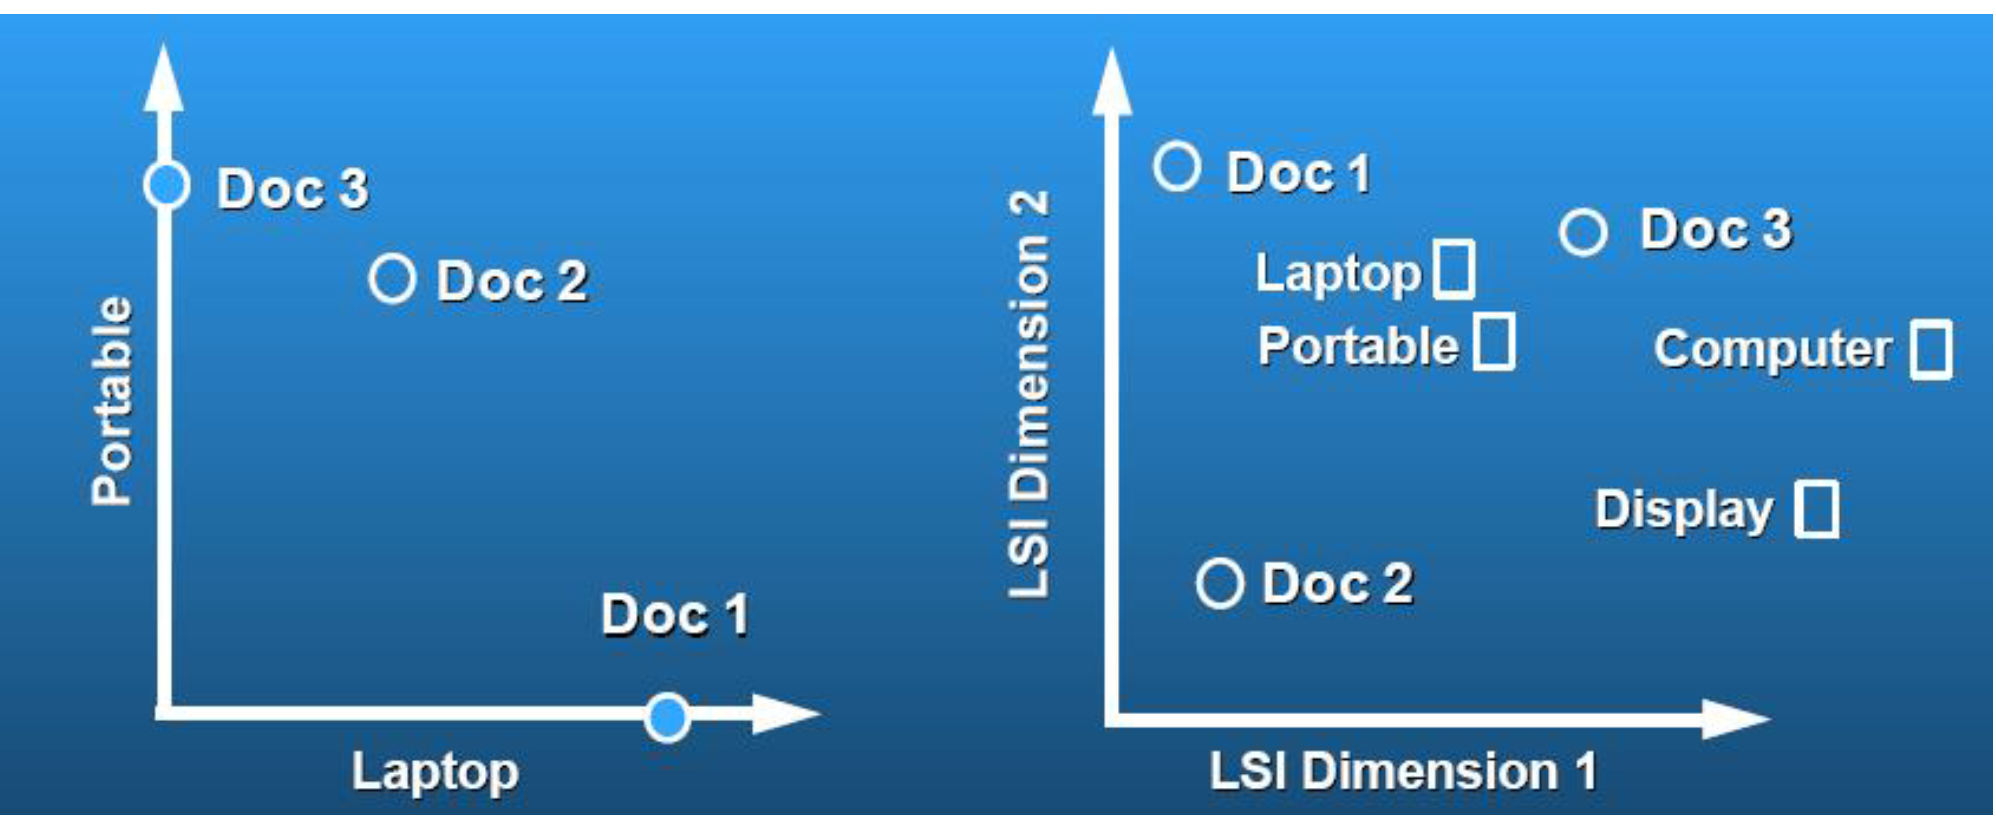
\includegraphics{img/lsa.png}
\caption{lsa}
\end{figure}

Grafik von Susan Dumais, siehe Präsentation.

    Das Ziel der LSA ist es, die Konzepte innerhalb der Dokumente zu finden.
Dabei greift das Verfahren auf eine Technik der linearen Algebra zurück,
der \textbf{Singulärwertzerlegung} (englisch: Singular Value
Decomposition). Die Idee dabei ist, dass die Term-Dokument Matrix aus
\textbf{Hauptdimensionen}, welche die wichtigen Konzepte der Dokumente
beinhalten, und aus weniger aussagekräftigen Dimensionen mit unwichtigen
Termen besteht. Mithilfe der Singulärwertzerlegung wird die originale
Term-Dokument Matrix in drei Matrizen aufgeteilt, wobei die beiden
äußeren Matrizen aus den linken bzw. rechten orthonormalen Eigenvektoren
bestehen und die mittlere Matrix eine Diagonalmatrix ist, die die
singulären Werte der Originalmatrix enthält. Mit Hilfe dieser Zerlegung
kann eine \textbf{Approximation} der Originalmatrix mit einer kleiner
dimensionierten Matrix erreicht werden. Die singulären Werte in der
Diagonalmatrix sind nach ihrer Größe absteigend geordnet. Singulärwerte,
die unter einem bestimmten Schwellenwert liegen, werden entfernt. Auch
in den anderen Matrizen werden entsprechende Zeilen oder Spalten
entfernt. Mit Hilfe der reduzierten Matrizen erhält man durch
Matrixmultiplikation die optimale Approximation der Originalmatrix, die
kleiner als die originale Term-Dokument Matrix ist, da Informationen aus
den weniger aussagekräftigen Dimensionen verworfen wurden. Weiterhin
werden bei der Dimensionsreduktion auch ähnliche Konzepte
zusammengefasst, so werden z.B. Worte wie ``Tür'' und ``Tor'' in einem
Konzept zusammengefasst.

Der Vorteil der LSA ist, dass anders als beim Bag-of-Words Modell die
\textbf{Semantik} der Dokumente wiedergegeben werden kann. Zudem werden
\textbf{Synonyme} zusammengefasst. Probleme hat LSA jedoch mit der
\textbf{Polysemie}. Zudem ist der Algorithmus sehr rechenaufwendig.

TODO: mehr?

    \hypertarget{word-embeddings}{%
\section{Word Embeddings}\label{word-embeddings}}

\hypertarget{allgemeines}{%
\subsection{Allgemeines}\label{allgemeines}}

\textbf{Word Embeddings} (deutsch: Worteinbettungen) sind die
Sammelbezeichnung für eine Reihe von Sprachmodellierungstechniken.
Anders als beim Bag-of-Words Modell werden Wörter mit ähnlichen
Bedeutungen ähnlich dargestellt, wobei der Kontext der Wörter
berücksichtigt wird. Word Embeddings repräsentieren Wörter als Vektoren
in einem multidimensionalen semantischen Raum. In diesem Raum werden
Wörter, die ähnlich zueinander sind, näher beieinander platziert. Diesen
Raum kann man sich etwa folgendermaßen vorstellen:

\begin{figure}
\centering
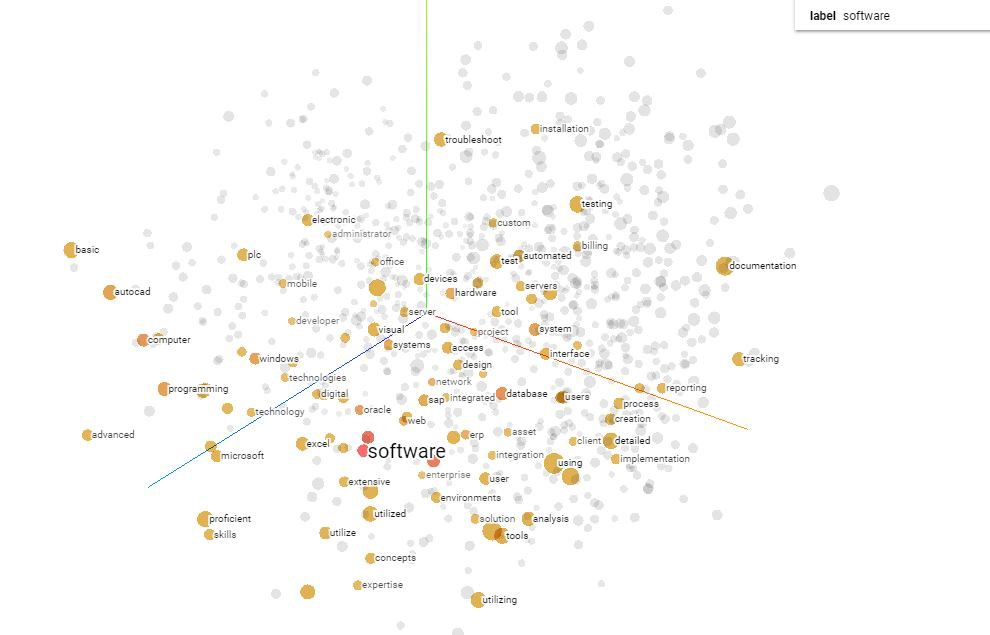
\includegraphics{img/we_space.jpg}
\caption{wordembeddings}
\end{figure}

    Die grundsätzliche Idee von Word Embeddings basiert auf der
\textbf{Distributionellen Hypothese} von John Rupert Firth, die besagt,
dass die Bedeutung eines Wortes durch sein Umfeld geprägt ist. Wörter,
die einen ähnlichen Kontext besitzen, haben eine ähnliche Bedeutung.
Anders als vorherige Vektorisierungsmethoden basieren Word Embeddings
auf \textbf{Vorhersage-Modellen} (englisch: \textbf{prediction models}),
indem Wörter durch Wahrscheinlichkeiten anstatt durch Häufigkeiten wie
beim Bag-of-Words Modell oder bei der Latent Semantic Analysis
dargestellt werden. Weiterhin sind die Wortvektoren von Word Embeddings
anders als beim Bag-of-Words Modell \textbf{dichtbesetzt} (englisch:
\textbf{dense}) und haben weitaus weniger Dimensionen (100-800
Dimensionen anstatt 100000-1000000, je nach der Größe des Vokabulars).
Dadurch haben die Wortvektoren eine viel geringere Größe, bieten
trotzdem eine effizientere und komplexere Darstellung der Wörter.

Eine weitere Besonderheit von Word Embeddings ist, dass es mit diesen
möglich ist, eine Arithmetik mit Wörtern umzusetzen. So kann mit
Wortvektoren ``gerechnet'' werden. Folgende Gleichungen sind mit Word
Embeddings möglich:

\texttt{König\ -\ Mann\ +\ Frau\ =\ Königin}

\texttt{London\ -\ Großbritannien\ +\ Deutschland\ =\ Berlin}

Word Embeddings wurden ab 2013 durch die Einführung des Algorithmus
\textbf{Word2Vec} populär, in den Jahren darauf folgten weitere Word
Embedding Algorithmen wie \textbf{GloVe}, \textbf{FastText},
\textbf{ELMo} und \textbf{BERT}. In der folgenden Tabelle sind die
wichtigsten Unterschiede der verschiedenen Embeddings zusammengefasst,
genauere Erläuterungen der Embeddings befinden sich in den folgenden
Kapiteln.

    TODO: ausfüllen \& mehr, gucken wie anders dargestellt werden kann

Word2Vec

GloVe

FastText

ELMo

BERT

Entstehungsjahr

2013

2014

2016

2018

2018

Out of vocabulary Fehler

ja

ja

nein

nein

nein

Kontextsensitiv

nein

nein

nein

ja

ja

    \hypertarget{word2vec}{%
\subsection{Word2Vec}\label{word2vec}}

Die Popularität von Word Embeddings ist vor allem \textbf{Word2Vec}
geschuldet, welches 2013 von Tomas Mikolov und weiteren Mitgliedern von
Google publiziert wurde. Word2Vec basiert auf einer simplen und
effektiven Feedforward Neuronalen Netzstruktur. Word2Vec implementiert
zwei verschiedene Ansätze zur Berechnung der Wortwahrscheinlichkeiten:
\textbf{Continous Bag of Words} (\textbf{CBOW}) und das
\textbf{Skip-gram Modell}.

\textbf{Continous Bag of Words} versucht die Wahrscheinlichkeit eines
Wortes oder einer Gruppe von Wörtern anhand eines gegebenen Kontext
vorauszusagen:

\begin{figure}
\centering
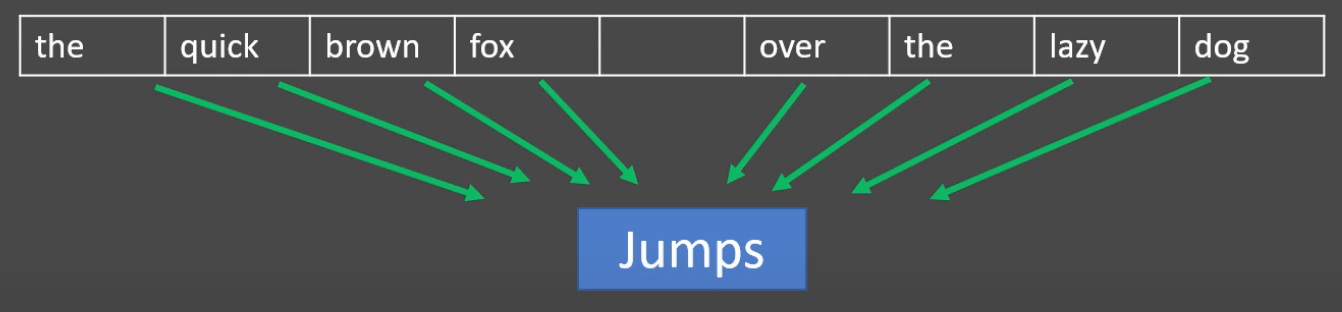
\includegraphics{img/cbow.png}
\caption{cbow}
\end{figure}

Das \textbf{Skip-gram Model} funktioniert wie CBOW, nur anders herum.
Das Modell versucht, anhand eines gegebenen Wortes den Kontext
vorauszusagen:

\begin{figure}
\centering
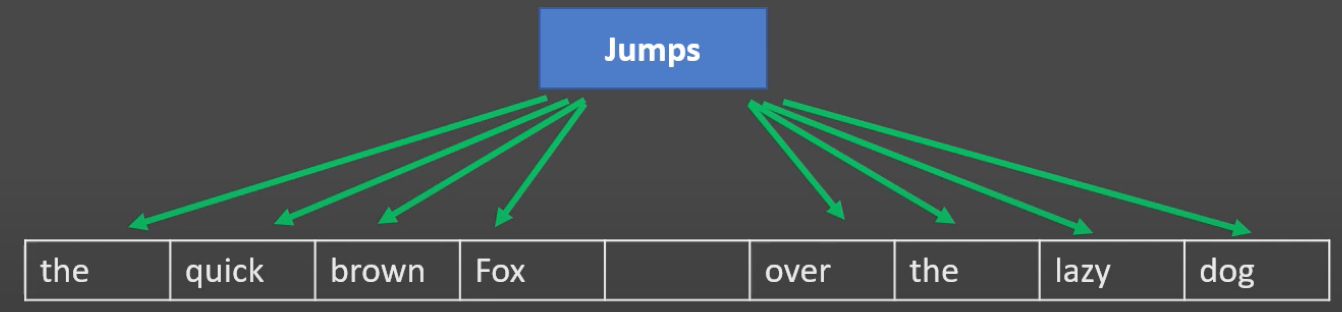
\includegraphics{img/skipgram.png}
\caption{skip-gram}
\end{figure}

Word2Vec nutzt wahlweise eine dieser Techniken, um aus rohen Textdaten
mithilfe eines Neuronales Netzes Wortvektoren zu erstellen. Dabei kann
Word2Vec bei vielen Implementierungen (z.b. bei Gensim) auf zwei Arten
verwendet werden: Entweder werden bereits vortrainierte Embeddings
geladen oder es werden eigene Embeddings auf eigenen Textdaten
trainiert.

    \hypertarget{vortrainierte-embeddings-verwenden}{%
\subsubsection{Vortrainierte Embeddings
verwenden}\label{vortrainierte-embeddings-verwenden}}

Für die Demonstration der Nutzung von vortrainierten Word Embeddings
wird ein deutsches Modell verwendet, welches auf Wikipedia- und
Zeitungsartikeln trainiert wurde
(\href{https://devmount.github.io/GermanWordEmbeddings/}{Quelle}). Als
Framework wird \textbf{Gensim} verwendet.

    \begin{tcolorbox}[breakable, size=fbox, boxrule=1pt, pad at break*=1mm,colback=cellbackground, colframe=cellborder]
\prompt{In}{incolor}{8}{\boxspacing}
\begin{Verbatim}[commandchars=\\\{\}]
\PY{n}{pre\PYZus{}w2v} \PY{o}{=} \PY{n}{gensim}\PY{o}{.}\PY{n}{models}\PY{o}{.}\PY{n}{KeyedVectors}\PY{o}{.}\PY{n}{load\PYZus{}word2vec\PYZus{}format}\PY{p}{(}\PY{l+s+s1}{\PYZsq{}}\PY{l+s+s1}{german\PYZus{}model.bin}\PY{l+s+s1}{\PYZsq{}}\PY{p}{,} 
                                                          \PY{n}{binary}\PY{o}{=}\PY{k+kc}{True}\PY{p}{)}
\end{Verbatim}
\end{tcolorbox}

    Im folgenden Code werden die 10 ähnlichsten Wörter zu ``König''
ausgegeben. Alle diese Wörter passen auch thematisch zu ``König'', sie
verbindet alle das Thema ``royal'' bzw. ``Königshaus''.

    \begin{tcolorbox}[breakable, size=fbox, boxrule=1pt, pad at break*=1mm,colback=cellbackground, colframe=cellborder]
\prompt{In}{incolor}{9}{\boxspacing}
\begin{Verbatim}[commandchars=\\\{\}]
\PY{k}{for} \PY{n}{t} \PY{o+ow}{in} \PY{n}{pre\PYZus{}w2v}\PY{o}{.}\PY{n}{most\PYZus{}similar}\PY{p}{(}\PY{l+s+s1}{\PYZsq{}}\PY{l+s+s1}{Koenig}\PY{l+s+s1}{\PYZsq{}}\PY{p}{,} \PY{n}{topn}\PY{o}{=}\PY{l+m+mi}{5}\PY{p}{)}\PY{p}{:} 
    \PY{n+nb}{print}\PY{p}{(}\PY{l+s+sa}{f}\PY{l+s+s2}{\PYZdq{}}\PY{l+s+si}{\PYZob{}}\PY{n}{t}\PY{p}{[}\PY{l+m+mi}{0}\PY{p}{]}\PY{l+s+si}{\PYZcb{}}\PY{l+s+s2}{: }\PY{l+s+si}{\PYZob{}}\PY{n}{np}\PY{o}{.}\PY{n}{around}\PY{p}{(}\PY{n}{t}\PY{p}{[}\PY{l+m+mi}{1}\PY{p}{]}\PY{p}{,} \PY{n}{decimals}\PY{o}{=}\PY{l+m+mi}{3}\PY{p}{)}\PY{l+s+si}{\PYZcb{}}\PY{l+s+s2}{\PYZdq{}}\PY{p}{)}
\end{Verbatim}
\end{tcolorbox}

    \begin{Verbatim}[commandchars=\\\{\}]
Prinz: 0.786
Koenigs: 0.736
Koenigin: 0.726
Jungkoenig: 0.705
Kaiser: 0.705
    \end{Verbatim}

    Auch das Rechenbeispiel aus Kapitel 3.1 TODO kann mit Word2Vec umgesetzt
werden. Addiert man ``König'' mit ``Frau'' und subtrahiert ``Mann'',
erhält man Begriffe zum Thema ``Königin''.

    \begin{tcolorbox}[breakable, size=fbox, boxrule=1pt, pad at break*=1mm,colback=cellbackground, colframe=cellborder]
\prompt{In}{incolor}{13}{\boxspacing}
\begin{Verbatim}[commandchars=\\\{\}]
\PY{k}{for} \PY{n}{t} \PY{o+ow}{in} \PY{n}{pre\PYZus{}w2v}\PY{o}{.}\PY{n}{most\PYZus{}similar}\PY{p}{(}\PY{n}{positive}\PY{o}{=}\PY{p}{[}\PY{l+s+s1}{\PYZsq{}}\PY{l+s+s1}{Koenig}\PY{l+s+s1}{\PYZsq{}}\PY{p}{,} \PY{l+s+s1}{\PYZsq{}}\PY{l+s+s1}{Frau}\PY{l+s+s1}{\PYZsq{}}\PY{p}{]}\PY{p}{,}
                              \PY{n}{negative}\PY{o}{=}\PY{p}{[}\PY{l+s+s1}{\PYZsq{}}\PY{l+s+s1}{Mann}\PY{l+s+s1}{\PYZsq{}}\PY{p}{]}\PY{p}{,} \PY{n}{topn}\PY{o}{=}\PY{l+m+mi}{5}\PY{p}{)}\PY{p}{:}
    \PY{n+nb}{print}\PY{p}{(}\PY{l+s+sa}{f}\PY{l+s+s2}{\PYZdq{}}\PY{l+s+si}{\PYZob{}}\PY{n}{t}\PY{p}{[}\PY{l+m+mi}{0}\PY{p}{]}\PY{l+s+si}{\PYZcb{}}\PY{l+s+s2}{: }\PY{l+s+si}{\PYZob{}}\PY{n}{np}\PY{o}{.}\PY{n}{around}\PY{p}{(}\PY{n}{t}\PY{p}{[}\PY{l+m+mi}{1}\PY{p}{]}\PY{p}{,} \PY{n}{decimals}\PY{o}{=}\PY{l+m+mi}{3}\PY{p}{)}\PY{l+s+si}{\PYZcb{}}\PY{l+s+s2}{\PYZdq{}}\PY{p}{)}
\end{Verbatim}
\end{tcolorbox}

    \begin{Verbatim}[commandchars=\\\{\}]
Koenigin: 0.752
Prinzessin: 0.715
Prinz: 0.688
Jungschuetzenkoenigin: 0.674
Majestaet: 0.659
    \end{Verbatim}

    Weiterhin kann man auch ein Wort mit einer Liste von anderen Wörtern
vergleichen und abfragen, welchem Wort aus der Liste das Wort am
ähnlichsten ist oder man überprüft bei einer Liste von Wörtern, welches
Wort nicht passt.

    \begin{tcolorbox}[breakable, size=fbox, boxrule=1pt, pad at break*=1mm,colback=cellbackground, colframe=cellborder]
\prompt{In}{incolor}{20}{\boxspacing}
\begin{Verbatim}[commandchars=\\\{\}]
\PY{n}{most\PYZus{}similar} \PY{o}{=} \PY{n}{pre\PYZus{}w2v}\PY{o}{.}\PY{n}{most\PYZus{}similar\PYZus{}to\PYZus{}given}\PY{p}{(}\PY{l+s+s1}{\PYZsq{}}\PY{l+s+s1}{Banane}\PY{l+s+s1}{\PYZsq{}}\PY{p}{,} \PY{p}{[}\PY{l+s+s1}{\PYZsq{}}\PY{l+s+s1}{Koenig}\PY{l+s+s1}{\PYZsq{}}\PY{p}{,} \PY{l+s+s1}{\PYZsq{}}\PY{l+s+s1}{Berg}\PY{l+s+s1}{\PYZsq{}}\PY{p}{,} 
                                                        \PY{l+s+s1}{\PYZsq{}}\PY{l+s+s1}{Haus}\PY{l+s+s1}{\PYZsq{}}\PY{p}{,} \PY{l+s+s1}{\PYZsq{}}\PY{l+s+s1}{Apfel}\PY{l+s+s1}{\PYZsq{}}\PY{p}{]}\PY{p}{)}
\PY{n}{doesnt\PYZus{}match} \PY{o}{=} \PY{n}{pre\PYZus{}w2v}\PY{o}{.}\PY{n}{doesnt\PYZus{}match}\PY{p}{(}\PY{p}{[}\PY{l+s+s1}{\PYZsq{}}\PY{l+s+s1}{Koenig}\PY{l+s+s1}{\PYZsq{}}\PY{p}{,} \PY{l+s+s1}{\PYZsq{}}\PY{l+s+s1}{Thron}\PY{l+s+s1}{\PYZsq{}}\PY{p}{,} \PY{l+s+s1}{\PYZsq{}}\PY{l+s+s1}{Berg}\PY{l+s+s1}{\PYZsq{}}\PY{p}{,} \PY{l+s+s1}{\PYZsq{}}\PY{l+s+s1}{Prinzessin}\PY{l+s+s1}{\PYZsq{}}\PY{p}{]}\PY{p}{)}
\PY{n+nb}{print}\PY{p}{(}\PY{l+s+sa}{f}\PY{l+s+s2}{\PYZdq{}}\PY{l+s+s2}{Welches Wort ist am ähnlichsten zu }\PY{l+s+s2}{\PYZsq{}}\PY{l+s+s2}{Banane}\PY{l+s+s2}{\PYZsq{}}\PY{l+s+s2}{? \PYZhy{}\PYZgt{} }\PY{l+s+si}{\PYZob{}}\PY{n}{most\PYZus{}similar}\PY{l+s+si}{\PYZcb{}}\PY{l+s+s2}{\PYZdq{}}\PY{p}{)}
\PY{n+nb}{print}\PY{p}{(}\PY{l+s+sa}{f}\PY{l+s+s2}{\PYZdq{}}\PY{l+s+s2}{Welches Wort nicht zu den anderen Wörtern? \PYZhy{}\PYZgt{} }\PY{l+s+si}{\PYZob{}}\PY{n}{doesnt\PYZus{}match}\PY{l+s+si}{\PYZcb{}}\PY{l+s+s2}{\PYZdq{}}\PY{p}{)}
\end{Verbatim}
\end{tcolorbox}

    \begin{Verbatim}[commandchars=\\\{\}]
Welches Wort ist am ähnlichsten zu 'Banane'? -> Apfel
Welches Wort nicht zu den anderen Wörtern? -> Berg
    \end{Verbatim}

    Die Wortvektoren können mit verwandeten Wörtern (hier die 5 ähnlichsten
Wörter) auch geplottet werden, wodurch die einzelnen Themen sehr gut
sichtbar sind.

    \begin{tcolorbox}[breakable, size=fbox, boxrule=1pt, pad at break*=1mm,colback=cellbackground, colframe=cellborder]
\prompt{In}{incolor}{12}{\boxspacing}
\begin{Verbatim}[commandchars=\\\{\}]
\PY{n}{wordlist} \PY{o}{=} \PY{p}{[}\PY{l+s+s1}{\PYZsq{}}\PY{l+s+s1}{Haus}\PY{l+s+s1}{\PYZsq{}}\PY{p}{,} \PY{l+s+s1}{\PYZsq{}}\PY{l+s+s1}{Berg}\PY{l+s+s1}{\PYZsq{}}\PY{p}{,} \PY{l+s+s1}{\PYZsq{}}\PY{l+s+s1}{Koenig}\PY{l+s+s1}{\PYZsq{}}\PY{p}{,} \PY{l+s+s1}{\PYZsq{}}\PY{l+s+s1}{gehen}\PY{l+s+s1}{\PYZsq{}}\PY{p}{]}
\PY{n}{plot\PYZus{}word\PYZus{}embeddings}\PY{p}{(}\PY{n}{pre\PYZus{}w2v}\PY{p}{,} \PY{n}{wordlist}\PY{p}{,} \PY{n}{figsize}\PY{o}{=}\PY{p}{(}\PY{l+m+mi}{8}\PY{p}{,}\PY{l+m+mi}{4}\PY{p}{)}\PY{p}{)}
\end{Verbatim}
\end{tcolorbox}

    \begin{center}
    \adjustimage{max size={0.9\linewidth}{0.9\paperheight}}{output_27_0.png}
    \end{center}
    { \hspace*{\fill} \\}
    
    \hypertarget{eigene-embeddings-trainieren}{%
\subsubsection{Eigene Embeddings
trainieren}\label{eigene-embeddings-trainieren}}

Es ist auch möglich, eigene Embeddings zu trainieren. Dabei muss sich
zuvor für die Technik \textbf{CBOW} oder \textbf{Skip-gram} entschieden
werden (wird durch den Parameter \texttt{sg}gesteuert). Es wurde der
englische Datensatz \textbf{Amazon Reviews} verwendet
(\href{https://nijianmo.github.io/amazon/index.html}{Quelle}). Dieser
wurde für Demonstrationszwecke auf Reviews zu elektronischen Geräten aus
dem Jahr 2018 gekürzt. Auch hier passen die ähnlichsten 5 Wörter sehr
gut zum ausgewählten Wort \emph{smartphone}.

    \begin{tcolorbox}[breakable, size=fbox, boxrule=1pt, pad at break*=1mm,colback=cellbackground, colframe=cellborder]
\prompt{In}{incolor}{23}{\boxspacing}
\begin{Verbatim}[commandchars=\\\{\}]
\PY{o}{\PYZpc{}\PYZpc{}time}
\PY{n}{word2vec\PYZus{}cbow} \PY{o}{=} \PY{n}{Word2Vec}\PY{p}{(}\PY{n}{texts}\PY{p}{,} \PY{n}{min\PYZus{}count}\PY{o}{=}\PY{l+m+mi}{1}\PY{p}{,} \PY{n}{size}\PY{o}{=}\PY{l+m+mi}{100}\PY{p}{,} \PY{n}{window}\PY{o}{=}\PY{l+m+mi}{5}\PY{p}{,} \PY{n}{sg}\PY{o}{=}\PY{l+m+mi}{0}\PY{p}{)}
\PY{n}{word2vec\PYZus{}skipgram} \PY{o}{=} \PY{n}{Word2Vec}\PY{p}{(}\PY{n}{texts}\PY{p}{,} \PY{n}{min\PYZus{}count}\PY{o}{=}\PY{l+m+mi}{1}\PY{p}{,} \PY{n}{size}\PY{o}{=}\PY{l+m+mi}{100}\PY{p}{,} \PY{n}{window}\PY{o}{=}\PY{l+m+mi}{5}\PY{p}{,} \PY{n}{sg}\PY{o}{=}\PY{l+m+mi}{1}\PY{p}{)}
\end{Verbatim}
\end{tcolorbox}

    \begin{Verbatim}[commandchars=\\\{\}]
CPU times: user 6min 1s, sys: 4.19 s, total: 6min 5s
Wall time: 2min 53s
    \end{Verbatim}

    \begin{tcolorbox}[breakable, size=fbox, boxrule=1pt, pad at break*=1mm,colback=cellbackground, colframe=cellborder]
\prompt{In}{incolor}{26}{\boxspacing}
\begin{Verbatim}[commandchars=\\\{\}]
\PY{n}{word2vec\PYZus{}cbow}\PY{o}{.}\PY{n}{wv}\PY{o}{.}\PY{n}{most\PYZus{}similar}\PY{p}{(}\PY{l+s+s1}{\PYZsq{}}\PY{l+s+s1}{phone}\PY{l+s+s1}{\PYZsq{}}\PY{p}{,} \PY{n}{topn}\PY{o}{=}\PY{l+m+mi}{5}\PY{p}{)}
\end{Verbatim}
\end{tcolorbox}

            \begin{tcolorbox}[breakable, size=fbox, boxrule=.5pt, pad at break*=1mm, opacityfill=0]
\prompt{Out}{outcolor}{26}{\boxspacing}
\begin{Verbatim}[commandchars=\\\{\}]
[('iphone', 0.7408102750778198),
 ('phones', 0.657496452331543),
 ('ph', 0.635297954082489),
 ('car', 0.626123309135437),
 ('cell', 0.6212888956069946)]
\end{Verbatim}
\end{tcolorbox}
        
    \hypertarget{glove}{%
\subsection{GloVe}\label{glove}}

\textbf{GloVe} wurde 2014 von Pennigton et. al.~veröffentlicht. Vor der
Veröffentlichung von Globe ließen sich die Wortvektorisierungsmethoden
in zwei Hauptströmungen unterteilen: das Statistik-basierende
\textbf{LDA}Section \ref{fn2} und das lernbasierte \textbf{Word2Vec}.
Während LDA Wörter mithilfe von Häufigkeiten in einer Kookkurrenz-Matrix
darstellt, verwendet Word2Vec zur Darstellung der Wörter
Wortwahrscheinlichkeiten, die mithilfe eines Voraussage-Modells erstellt
wurden. \textbf{GloVe} verwendet wie LDA für die Darstellung der
Häufigkeiten eine Kookkurrenz-Matrix, wobei GloVe die Häufigkeiten
vorher normalisiert und mithilfe des Logarithmus \emph{``glättet''}
(englisch: \emph{smoothing}). Anders als Word2Vec benutzt es für die
Erstellung der Embeddings also keine neuronalen Netze

\hypertarget{fn1}{}
2 ~LDA steht für ``Latent Dirichlet allocation'' und ist ein
Algorithmus, der Wörter ähnlichen Gruppen anhand der Wahrscheinlichkeit,
dass sie zusammen in einem Dokument vorkommen, zuordnet.

    \begin{tcolorbox}[breakable, size=fbox, boxrule=1pt, pad at break*=1mm,colback=cellbackground, colframe=cellborder]
\prompt{In}{incolor}{ }{\boxspacing}
\begin{Verbatim}[commandchars=\\\{\}]

\end{Verbatim}
\end{tcolorbox}

    Beide Modelle lernen geometrische Kodierungen (Vektoren) von Wörtern aus
ihren Informationen über das gleichzeitige Vorkommen (wie häufig sie
zusammen in großen Textkorpora vorkommen). Sie unterscheiden sich darin,
dass word2vec ein ``prädiktives'' Modell ist, während GloVe ein
``zählbasiertes'' Modell ist. Weitere Informationen zu den Unterschieden
zwischen diesen beiden Ansätzen finden Sie in diesem Papier: .
Prädiktive Modelle lernen ihre Vektoren, um ihre Fähigkeit zur
Vorhersage von Verlust(Zielwort \textbar{} Kontextwörter; Vektoren) zu
verbessern, d.h. den Verlust der Vorhersage der Zielwörter aus den
Kontextwörtern angesichts der Vektordarstellungen. In word2vec wird dies
als Feed-Forward Neuronales Netz gegossen und als solches mittels SGD
etc. optimiert. Zählbasierte Modelle lernen ihre Vektoren, indem sie im
Wesentlichen eine Dimensionalitätsreduktion auf der
Koinzidenz-Zählmatrix durchführen. Zuerst konstruieren sie eine große
Matrix von (Wörter x Kontext) Ko-Vorkommensinformationen, d.h. für jedes
``Wort'' (die Zeilen) wird gezählt, wie oft wir dieses Wort in einem
``Kontext'' (den Spalten) in einem großen Korpus sehen. Die Anzahl der
``Kontexte'' ist natürlich groß, da sie im Wesentlichen kombinatorisch
ist. Dann faktorisieren sie also diese Matrix, um eine
niedrigdimensionale (Wort x Merkmale) Matrix zu erhalten, wobei jede
Zeile nun eine Vektordarstellung für jedes Wort ergibt. Im Allgemeinen
geschieht dies durch Minimierung eines ``Rekonstruktionsverlustes'', der
versucht, die niedrigdimensionalen Darstellungen zu finden, die den
größten Teil der Varianz in den hochdimensionalen Daten erklären können.
Im speziellen Fall von GloVe wird die Zählmatrix vorverarbeitet, indem
die Zählwerte normalisiert und logarithmisch geglättet werden. Dies
erweist sich als eine gute Sache im Hinblick auf die Qualität der
gelernten Darstellungen. Wie bereits erwähnt, neigen jedoch, wenn wir
alle Trainings-Hyperparameter kontrollieren, die Einbettungen, die mit
den beiden Methoden erzeugt werden, dazu, bei nachgeschalteten
NLP-Aufgaben sehr ähnlich zu funktionieren. Der zusätzliche Vorteil von
GloVe gegenüber word2vec besteht darin, dass es einfacher ist, die
Implementierung zu parallelisieren, was bedeutet, dass es einfacher ist,
über mehr Daten zu trainieren, was bei diesen Modellen immer eine gute
Sache ist. Übersetzt mit www.DeepL.com/Translator (kostenlose Version)

    \begin{tcolorbox}[breakable, size=fbox, boxrule=1pt, pad at break*=1mm,colback=cellbackground, colframe=cellborder]
\prompt{In}{incolor}{ }{\boxspacing}
\begin{Verbatim}[commandchars=\\\{\}]

\end{Verbatim}
\end{tcolorbox}

    Um diese Frage besser zu erklären, möchte ich zum Vergleich die LDA mit
einbeziehen. Vor GloVe lassen sich die Algorithmen von Wortdarstellungen
in zwei Hauptströme unterteilen, den statistikbasierten (LDA) und den
lernbasierten (Word2Vec). LDA erzeugt die niedrigdimensionalen
Wortvektoren durch Singulärwertzerlegung (SVD) auf der
Ko-Vorkommensmatrix, während Word2Vec ein dreischichtiges neuronales
Netz verwendet, um die Aufgabe der Wortpaarklassifizierung im
Zentrumskontext zu erledigen, wobei die Wortvektoren nur das
Nebenprodukt sind.

Der erstaunlichste Punkt von Word2Vec ist, dass ähnliche Wörter zusammen
im Vektorraum liegen und arithmetische Operationen auf Wortvektoren
semantische oder syntaktische Beziehungen herstellen können, z.B.
``König'' - ``Mann'' + ``Frau'' -\textgreater{} ``Königin'' oder
``besser'' - ``gut'' + ``schlecht'' -\textgreater{} ``schlechter''.
Allerdings kann die LDA eine solche lineare Beziehung im Vektorraum
nicht aufrechterhalten.

Die Motivation von GloVe besteht darin, das Modell zu zwingen, eine
solche lineare Beziehung auf der Grundlage der Koinzidenzmatrix explizit
zu erlernen. Im Wesentlichen ist GloVe ein log-bilineares Modell mit
einem gewichteten Ziel der kleinsten Quadrate. Offensichtlich handelt es
sich um eine hybride Methode, die maschinelles Lernen auf der Grundlage
der statistischen Matrix verwendet, und dies ist der allgemeine
Unterschied zwischen GloVe und Word2Vec.

Wenn wir in das Deduktionsverfahren der Gleichungen in GloVe eintauchen,
werden wir den Unterschied in der Intuition finden. GloVe stellt fest,
dass die Verhältnisse der Wort-Wort-Koinzidenzwahrscheinlichkeiten das
Potenzial haben, irgendeine Form von Bedeutung zu kodieren. Nehmen wir
das Beispiel aus StanfordNLP (Global Vectors for Word Representation),
um die Ko-Vorkommenswahrscheinlichkeiten für die Zielwörter Eis und
Dampf mit verschiedenen Probewörtern aus dem Vokabular zu betrachten:

``Wie zu erwarten ist, tritt Eis häufiger mit Festkörpern als mit Gas
auf, während Dampf häufiger mit Gas als mit Festkörpern auftritt. Beide
Wörter kommen häufig zusammen mit ihrer gemeinsamen Eigenschaft Wasser
vor, und beide kommen selten zusammen mit dem nicht verwandten Wort Mode
vor. Nur im Verhältnis der Wahrscheinlichkeiten heben sich Geräusche von
nicht diskriminierenden Wörtern wie Wasser und Mode auf, so dass große
Werte (viel größer als 1) gut mit eisspezifischen Eigenschaften und
kleine Werte (viel kleiner als 1) gut mit dampfspezifischen
Eigenschaften korrelieren.'' Word2Vec arbeitet jedoch mit den reinen
Koinzidenzwahrscheinlichkeiten, so dass die Wahrscheinlichkeit, dass die
das Zielwort umgebenden Wörter den Kontext bilden, maximiert wird.

In der Praxis setzt Word2Vec zur Beschleunigung des Trainingsprozesses
negative Abtastung ein, um die Softmax-Funktion durch die
Sigmoid-Funktion zu ersetzen, die mit den realen Daten und den
Rauschdaten arbeitet. Dies führt emplizit zu einer Clusterung von
Wörtern zu einem Kegel im Vektorraum, während die Wortvektoren von GloVe
diskreter angeordnet sind. Übersetzt mit www.DeepL.com/Translator
(kostenlose Version)

    \hypertarget{fasttext}{%
\subsection{FastText}\label{fasttext}}

TODO

    \hypertarget{elmo}{%
\subsection{ELMo}\label{elmo}}

TODO

    \hypertarget{bert}{%
\subsection{BERT}\label{bert}}

BERT steht für ``Bidirectional Encoder Representations from
Transformers'' und brach bei seiner Veröffentlichung 2018 eine ganze
Reihe von Rekorden für Aufgaben des Natural Language Processing.

    \begin{tcolorbox}[breakable, size=fbox, boxrule=1pt, pad at break*=1mm,colback=cellbackground, colframe=cellborder]
\prompt{In}{incolor}{ }{\boxspacing}
\begin{Verbatim}[commandchars=\\\{\}]

\end{Verbatim}
\end{tcolorbox}


    % Add a bibliography block to the postdoc
    
    
    
\end{document}
